\documentclass{article}
\usepackage{graphicx,xcolor,tikz,amsmath,hyperref}
\usepackage[T1]{fontenc}
\usepackage{lmodern}
\begin{document}
\tableofcontents
\section{Images}\label{sec:img}
\includegraphics[width=\linewidth]{big-1.png}
\includegraphics[width=\linewidth]{photo-01.jpg}
See \ref{sec:tikz}, \url{https://example.org} and \href{mailto:a@b.c}{mail}.
\section{TikZ}\label{sec:tikz}
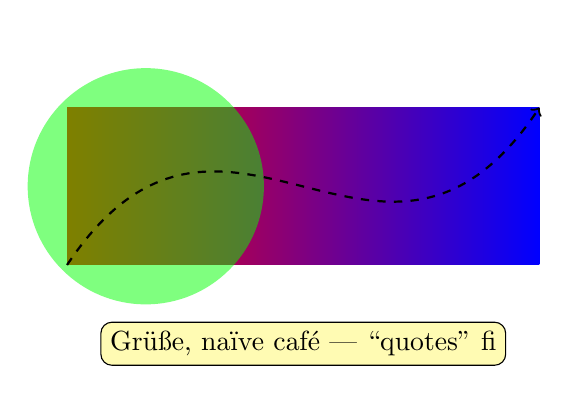
\begin{tikzpicture}
\shade[left color=red,right color=blue] (0,0) rectangle (6,2);
\fill[green,opacity=0.5] (1,1) circle (1.5);
\draw[dashed,thick,->] (0,0) .. controls (2,3) and (4,-1) .. (6,2);
\node[draw,rounded corners,fill=yellow!30] at (3,-1) {Grüße, naïve café — “quotes” fi};
\end{tikzpicture}
\foreach \i in {1,...,40}{\subsection{Part \i} Text with \textbf{bold} \emph{emph} \texttt{mono} and $\int_0^\infty e^{-x^2}\,dx=\frac{\sqrt\pi}{2}$. \par

\begin{tikzpicture}\foreach \j in {1,...,30}{\draw[color=blue!\j] (\j/5,0) -- (\j/5+1,1);}\end{tikzpicture}\newpage}
\end{document}
